\documentclass{standalone}
\usepackage{tikz}
\usetikzlibrary{patterns, positioning}


\begin{document}
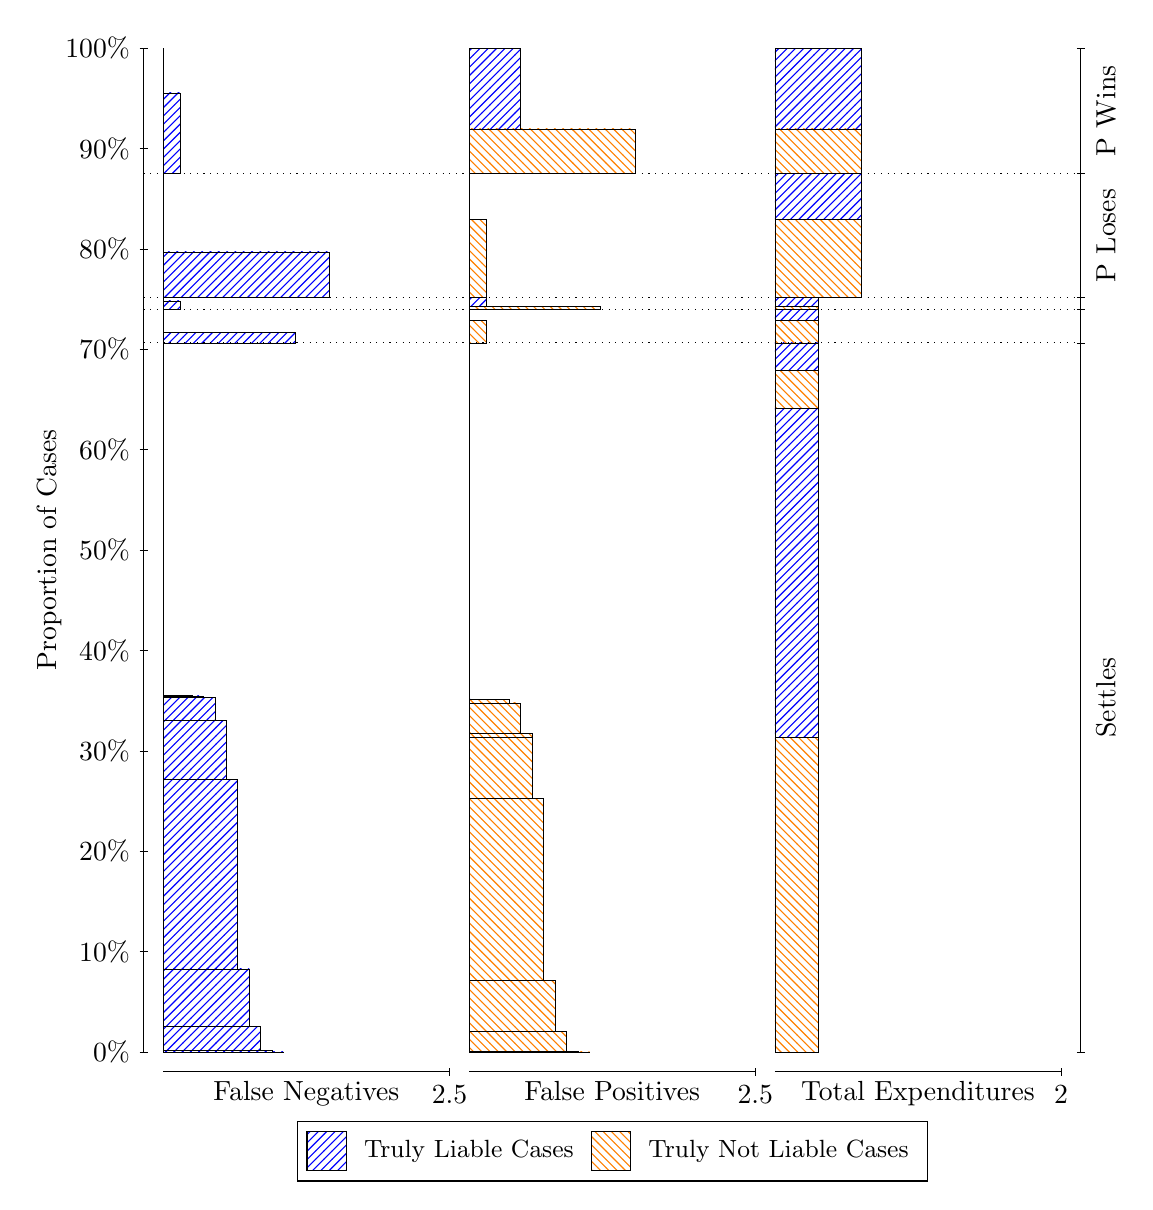
\begin{tikzpicture}
\draw[black, very thin] (1.5,1.75) -- (1.5,14.5);
\node[rotate=90, text=black, anchor=center] at (0.3, 8.125) {Proportion of Cases};
\draw[black, very thin] (1.45,1.75) -- (1.55,1.75);
\node[text=black, anchor=east] at (1.45, 1.75) {0\%};
\draw[black, very thin] (1.45,3.025) -- (1.55,3.025);
\node[text=black, anchor=east] at (1.45, 3.025) {10\%};
\draw[black, very thin] (1.45,4.3) -- (1.55,4.3);
\node[text=black, anchor=east] at (1.45, 4.3) {20\%};
\draw[black, very thin] (1.45,5.575) -- (1.55,5.575);
\node[text=black, anchor=east] at (1.45, 5.575) {30\%};
\draw[black, very thin] (1.45,6.85) -- (1.55,6.85);
\node[text=black, anchor=east] at (1.45, 6.85) {40\%};
\draw[black, very thin] (1.45,8.125) -- (1.55,8.125);
\node[text=black, anchor=east] at (1.45, 8.125) {50\%};
\draw[black, very thin] (1.45,9.4) -- (1.55,9.4);
\node[text=black, anchor=east] at (1.45, 9.4) {60\%};
\draw[black, very thin] (1.45,10.675) -- (1.55,10.675);
\node[text=black, anchor=east] at (1.45, 10.675) {70\%};
\draw[black, very thin] (1.45,11.95) -- (1.55,11.95);
\node[text=black, anchor=east] at (1.45, 11.95) {80\%};
\draw[black, very thin] (1.45,13.225) -- (1.55,13.225);
\node[text=black, anchor=east] at (1.45, 13.225) {90\%};
\draw[black, very thin] (1.45,14.5) -- (1.55,14.5);
\node[text=black, anchor=east] at (1.45, 14.5) {100\%};

\draw[black, very thin] (13.4,1.75) -- (13.4,14.5);
\draw[black, very thin] (13.35,1.75) -- (13.45,1.75);
\node[anchor=west] at (13.35, 1.75) {};
\draw[black, very thin] (13.35,10.756) -- (13.45,10.756);
\node[anchor=west] at (13.35, 10.756) {};
\draw[black, very thin] (13.35,11.177) -- (13.45,11.177);
\node[anchor=west] at (13.35, 11.177) {};
\draw[black, very thin] (13.35,11.331) -- (13.45,11.331);
\node[anchor=west] at (13.35, 11.331) {};
\draw[black, very thin] (13.35,12.905) -- (13.45,12.905);
\node[anchor=west] at (13.35, 12.905) {};
\draw[black, very thin] (13.35,14.5) -- (13.45,14.5);
\node[anchor=west] at (13.35, 14.5) {};

\draw[black, very thin, pattern color=blue, pattern=north east lines] (1.75,1.75) rectangle (3.276,1.7516);
\draw[black, very thin, pattern color=blue, pattern=north east lines] (1.75,1.7516) rectangle (3.1307,1.7741);
\draw[black, very thin, pattern color=blue, pattern=north east lines] (1.75,1.7741) rectangle (2.9853,2.0737);
\draw[black, very thin, pattern color=blue, pattern=north east lines] (1.75,2.0737) rectangle (2.84,2.805);
\draw[black, very thin, pattern color=blue, pattern=north east lines] (1.75,2.805) rectangle (2.6947,5.2134);
\draw[black, very thin, pattern color=blue, pattern=north east lines] (1.75,5.2134) rectangle (2.5493,5.9579);
\draw[black, very thin, pattern color=blue, pattern=north east lines] (1.75,5.9579) rectangle (2.404,6.2535);
\draw[black, very thin, pattern color=blue, pattern=north east lines] (1.75,6.2535) rectangle (2.2587,6.2725);
\draw[black, very thin, pattern color=blue, pattern=north east lines] (1.75,6.2725) rectangle (2.1133,6.274);
\draw[black, very thin, pattern color=orange, pattern=north west lines] (1.75,6.274) rectangle (1.75,10.756);
\draw[black, very thin, pattern color=blue, pattern=north east lines] (1.75,10.756) rectangle (3.4213,10.888);
\draw[black, very thin, pattern color=orange, pattern=north west lines] (1.75,10.888) rectangle (1.75,11.177);
\draw[black, very thin, pattern color=blue, pattern=north east lines] (1.75,11.177) rectangle (1.968,11.29);
\draw[black, very thin, pattern color=orange, pattern=north west lines] (1.75,11.29) rectangle (1.75,11.331);
\draw[black, very thin, pattern color=blue, pattern=north east lines] (1.75,11.331) rectangle (3.8573,11.911);
\draw[black, very thin, pattern color=orange, pattern=north west lines] (1.75,11.911) rectangle (1.75,12.905);
\draw[black, very thin, pattern color=blue, pattern=north east lines] (1.75,12.905) rectangle (1.968,13.931);
\draw[black, very thin, pattern color=orange, pattern=north west lines] (1.75,13.931) rectangle (1.75,14.5);
\draw[black, very thin, pattern color=orange, pattern=north west lines] (5.6333,1.75) rectangle (7.1593,1.7512);
\draw[black, very thin, pattern color=orange, pattern=north west lines] (5.6333,1.7512) rectangle (7.014,1.7585);
\draw[black, very thin, pattern color=orange, pattern=north west lines] (5.6333,1.7585) rectangle (6.8687,2.0137);
\draw[black, very thin, pattern color=orange, pattern=north west lines] (5.6333,2.0137) rectangle (6.7233,2.6618);
\draw[black, very thin, pattern color=orange, pattern=north west lines] (5.6333,2.6618) rectangle (6.578,4.9714);
\draw[black, very thin, pattern color=orange, pattern=north west lines] (5.6333,4.9714) rectangle (6.4327,5.7444);
\draw[black, very thin, pattern color=orange, pattern=north west lines] (5.6333,5.7444) rectangle (6.4327,5.7928);
\draw[black, very thin, pattern color=orange, pattern=north west lines] (5.6333,5.7928) rectangle (6.2873,6.1833);
\draw[black, very thin, pattern color=orange, pattern=north west lines] (5.6333,6.1833) rectangle (6.142,6.2305);
\draw[black, very thin, pattern color=orange, pattern=north west lines] (5.6333,6.2305) rectangle (5.9967,6.2317);
\draw[black, very thin, pattern color=blue, pattern=north east lines] (5.6333,6.2317) rectangle (5.706,6.2332);
\draw[black, very thin, pattern color=blue, pattern=north east lines] (5.6333,6.2332) rectangle (5.6333,10.756);
\draw[black, very thin, pattern color=orange, pattern=north west lines] (5.6333,10.756) rectangle (5.8513,11.045);
\draw[black, very thin, pattern color=blue, pattern=north east lines] (5.6333,11.045) rectangle (5.6333,11.177);
\draw[black, very thin, pattern color=orange, pattern=north west lines] (5.6333,11.177) rectangle (7.3047,11.219);
\draw[black, very thin, pattern color=blue, pattern=north east lines] (5.6333,11.219) rectangle (5.8513,11.331);
\draw[black, very thin, pattern color=orange, pattern=north west lines] (5.6333,11.331) rectangle (5.8513,12.325);
\draw[black, very thin, pattern color=blue, pattern=north east lines] (5.6333,12.325) rectangle (5.6333,12.905);
\draw[black, very thin, pattern color=orange, pattern=north west lines] (5.6333,12.905) rectangle (7.7407,13.474);
\draw[black, very thin, pattern color=blue, pattern=north east lines] (5.6333,13.474) rectangle (6.2873,14.5);
\draw[black, very thin, pattern color=orange, pattern=north west lines] (9.5167,1.75) rectangle (10.062,5.7444);
\draw[black, very thin, pattern color=blue, pattern=north east lines] (9.5167,5.7444) rectangle (10.062,9.9215);
\draw[black, very thin, pattern color=orange, pattern=north west lines] (9.5167,9.9215) rectangle (10.062,9.9228);
\draw[black, very thin, pattern color=blue, pattern=north east lines] (9.5167,9.9228) rectangle (10.062,9.9244);
\draw[black, very thin, pattern color=orange, pattern=north west lines] (9.5167,9.9244) rectangle (10.062,10.41);
\draw[black, very thin, pattern color=blue, pattern=north east lines] (9.5167,10.41) rectangle (10.062,10.756);
\draw[black, very thin, pattern color=orange, pattern=north west lines] (9.5167,10.756) rectangle (10.062,11.045);
\draw[black, very thin, pattern color=blue, pattern=north east lines] (9.5167,11.045) rectangle (10.062,11.177);
\draw[black, very thin, pattern color=orange, pattern=north west lines] (9.5167,11.177) rectangle (10.062,11.219);
\draw[black, very thin, pattern color=blue, pattern=north east lines] (9.5167,11.219) rectangle (10.062,11.331);
\draw[black, very thin, pattern color=orange, pattern=north west lines] (9.5167,11.331) rectangle (10.607,12.325);
\draw[black, very thin, pattern color=blue, pattern=north east lines] (9.5167,12.325) rectangle (10.607,12.905);
\draw[black, very thin, pattern color=orange, pattern=north west lines] (9.5167,12.905) rectangle (10.607,13.474);
\draw[black, very thin, pattern color=blue, pattern=north east lines] (9.5167,13.474) rectangle (10.607,14.5);
\draw[black, dotted] (1.5,10.756) -- (13.4,10.756);
\draw[black, dotted] (1.5,11.177) -- (13.4,11.177);
\draw[black, dotted] (1.5,11.331) -- (13.4,11.331);
\draw[black, dotted] (1.5,12.905) -- (13.4,12.905);
\draw[black, very thin] (1.75,1.5) -- (5.3833,1.5);
\node[text=black, anchor=north] at (3.5667, 1.5) {False Negatives};
\draw[black, very thin] (5.3833,1.45) -- (5.3833,1.55);
\node[text=black, anchor=north] at (5.3833, 1.45) {2.5};

\draw[black, very thin] (5.6333,1.5) -- (9.2667,1.5);
\node[text=black, anchor=north] at (7.45, 1.5) {False Positives};
\draw[black, very thin] (9.2667,1.45) -- (9.2667,1.55);
\node[text=black, anchor=north] at (9.2667, 1.45) {2.5};

\draw[black, very thin] (9.5167,1.5) -- (13.15,1.5);
\node[text=black, anchor=north] at (11.333, 1.5) {Total Expenditures};
\draw[black, very thin] (13.15,1.45) -- (13.15,1.55);
\node[text=black, anchor=north] at (13.15, 1.45) {2};

\node[text=black, centered, rotate=90] at (13.72, 6.2529) {Settles};


\node[text=black, centered, rotate=90] at (13.72, 12.118) {P Loses};
\node[text=black, centered, rotate=90] at (13.72, 13.702) {P Wins};

\draw (7.449999999999999,1.5) node[draw=none] (baseCoordinate) {};
\begin{scope}[align=center]
        \matrix[scale=0.5, draw=black, below=0.5cm of baseCoordinate, nodes={draw}, column sep=0.1cm]{
            \node[rectangle, draw, minimum width=0.5cm, minimum height=0.5cm, pattern color=blue, pattern=north east lines] {}; &
            \node[draw=none, font=\small, text=black] (B) {Truly Liable Cases}; &
            \node[rectangle, draw, minimum width=0.5cm, minimum height=0.5cm, pattern color=orange, pattern=north west lines] {}; &
            \node[draw=none, font=\small, text=black] (B) {Truly Not Liable Cases}; \\
            };
\end{scope}

\end{tikzpicture}
\end{document}